\documentclass{standalone}
\usepackage{tikz}
\usetikzlibrary{quantikz}

\begin{document}
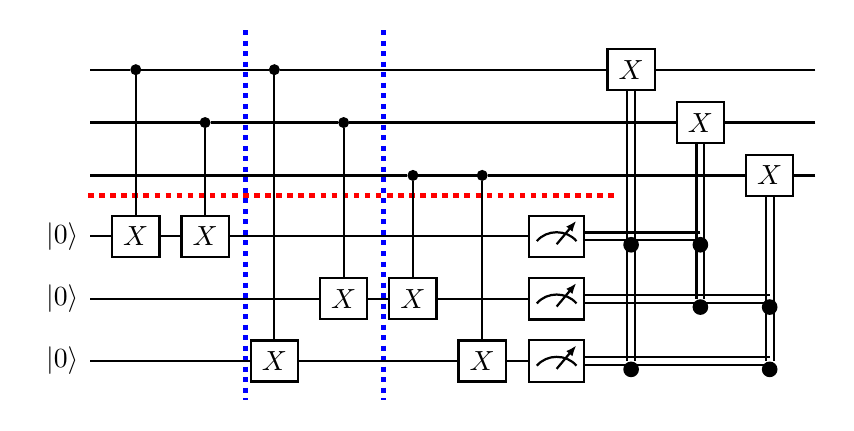
\begin{tikzpicture}
    \draw[dotted, red, line width =2pt] (-4.3,-2.1) -- (2.4,-2.1);
    \draw[dotted, blue, line width =1.8pt] (-2.3,0) -- (-2.3,-4.7);
    \draw[dotted, blue, line width =1.8pt] (-0.55,0) -- (-0.55,-4.7);
    \node at (0,0) [anchor=north]{
    \begin{quantikz}[column sep=0.28cm,row sep=0.15cm]%
                  &\ctrl{3}&\qw     &\ctrl{5}&\qw     &\qw     &\qw     &\qw     &\gate{X}&\qw&\qw&\qw \\
                  &\qw     &\ctrl{2}&\qw     &\ctrl{3}&\qw     &\qw     &\qw     &\qw&\gate{X}&\qw&\qw \\
                  &\qw     &\qw     &\qw     &\qw     &\ctrl{2}&\ctrl{3}&\qw     &\qw&\qw&\gate{X}&\qw \\
\lstick{$\ket{0}$}&\gate{X}&\gate{X}&\qw     &\qw     &\qw     &\qw     &\meter{}&\cwbend{-3}&\cwbend{-2} \\
\lstick{$\ket{0}$}&\qw     &\qw     &\qw     &\gate{X}&\gate{X}&\qw     &\meter{}&\cw&\cwbend{-1}&\cwbend{-2} \\
\lstick{$\ket{0}$}&\qw     &\qw     &\gate{X}&\qw     &\qw     &\gate{X}&\meter{}&\cwbend{-2}&\cw&\cwbend{-1}
    \end{quantikz}
    };
\end{tikzpicture}
\end{document}